\documentclass[letterpaper]{article}
\usepackage[submission]{aaai2026}
\usepackage{times}
\usepackage{helvet}
\usepackage{courier}
\usepackage[hyphens]{url}
\usepackage{graphicx}
\usepackage{amsmath}
\usepackage{amssymb}
\usepackage{amsthm}
\usepackage{booktabs}
\usepackage{natbib}
\usepackage{caption}
\frenchspacing
\pdfpagewidth=8.5in
\pdfpageheight=11in

\newtheorem{theorem}{Theorem}
\newtheorem{proposition}{Proposition}

\title{RC-Diff: Risk-Controlled Financial Diffusion with Path-Level Audits}
\author{PaperClaw}
\affiliations{Anonymous Institution}

\begin{document}
\maketitle

\begin{abstract}
Synthetic financial paths are useful only when their rare events and temporal structure are credible. Sequence generators can match marginal return histograms while missing volatility clustering, drawdown behavior, or the path ordering that makes a stress scenario economically meaningful. We study a compact diffusion generator for daily equity returns with an explicit volatility-conditioning channel, distributional risk calibration metrics, and signature-based path audits. On Yahoo Finance daily returns from S\&P 500 constituents, volatility conditioning gives strong monotone control over realized volatility: Spearman correlation between requested and realized volatility is 0.9788 with zero monotonicity violations, compared with 0.0171 and 0.5 violations for a conditional Sig-Wasserstein GAN proxy. More importantly, the conditioned diffusion improves absolute tail-risk calibration, reaching VaR and expected-shortfall calibration errors of 0.1454 and 0.0499, versus 0.3747 and 0.4145 for an unconditional diffusion and 0.9043 and 0.9162 for the Sig-Wasserstein GAN proxy. A separate path-audit experiment shows that depth-3 Mahalanobis signature distance detects temporal corruptions with AUC 0.5657, a 4.61\% relative improvement over the best marginal-only metric. A naive stylized-fact training loss, however, worsens tail-index error from 1.448 to 2.396, showing that risk-aware generation needs calibrated controls and audits, not indiscriminate moment penalties.
\end{abstract}

\section{Introduction}
Synthetic financial time series are increasingly used to stress test trading systems, validate risk models, augment scarce historical samples, and study counterfactual market regimes. The difficult cases are not ordinary trading days. A useful generator must reproduce heavy-tailed returns, volatility clustering, leverage effects, regime-dependent dependence, and drawdowns whose temporal ordering is economically meaningful \citep{mandelbrot1963variation,engle1982arch,bollerslev1986garch,cont2001stylized}. A path with the right marginal histogram but the wrong ordering can appear realistic under distributional tests while understating liquidation risk, breach clustering, or portfolio drawdown.

Classical financial modeling provides strong diagnostics for this problem but limited flexible generation. ARCH/GARCH families model conditional heteroskedasticity \citep{engle1982arch,bollerslev1986garch}, asymmetric volatility models capture leverage-like effects \citep{nelson1991egarch,glosten1993relation,engle1993measuring}, and stochastic-volatility models give latent volatility dynamics \citep{heston1993closed}. Extreme-value and risk-measure literatures formalize tail behavior, Value-at-Risk (VaR), expected shortfall (ES), and backtesting \citep{embrechts1997modelling,mcneil2015quantitative,artzner1999coherent,kupiec1995techniques,christoffersen1998evaluating,acerbi2002expected,fissler2016higher}. However, these tools usually specify a narrow parametric family rather than a high-dimensional scenario generator with controllable path properties.

Deep generative models relax this parametric restriction. Adversarial financial generators such as QuantGAN showed that neural models can synthesize continuous-valued return sequences \citep{wiese2020quant}. Diffusion and score-based models provide an alternative training paradigm with stable denoising objectives \citep{sohldickstein2015deep,ho2020ddpm,song2021score,nichol2021improved}. In finance, controllable diffusion models such as CoFinDiff point toward explicit condition interfaces for synthetic market data \citep{tanaka2025cofindiff}.

This paper asks a narrower question: can a financial diffusion model expose a risk-control interface that is both monotone and calibrated, while being audited by metrics that see path-level failures? We train compact one-dimensional U-Net DDPMs on rolling equity-return windows and condition them on target realized volatility. We evaluate not only rank monotonicity, but also VaR, expected shortfall, maximum drawdown, autocorrelation, tail-index error, and signature-style path distances.

\begin{figure}[t]
\centering
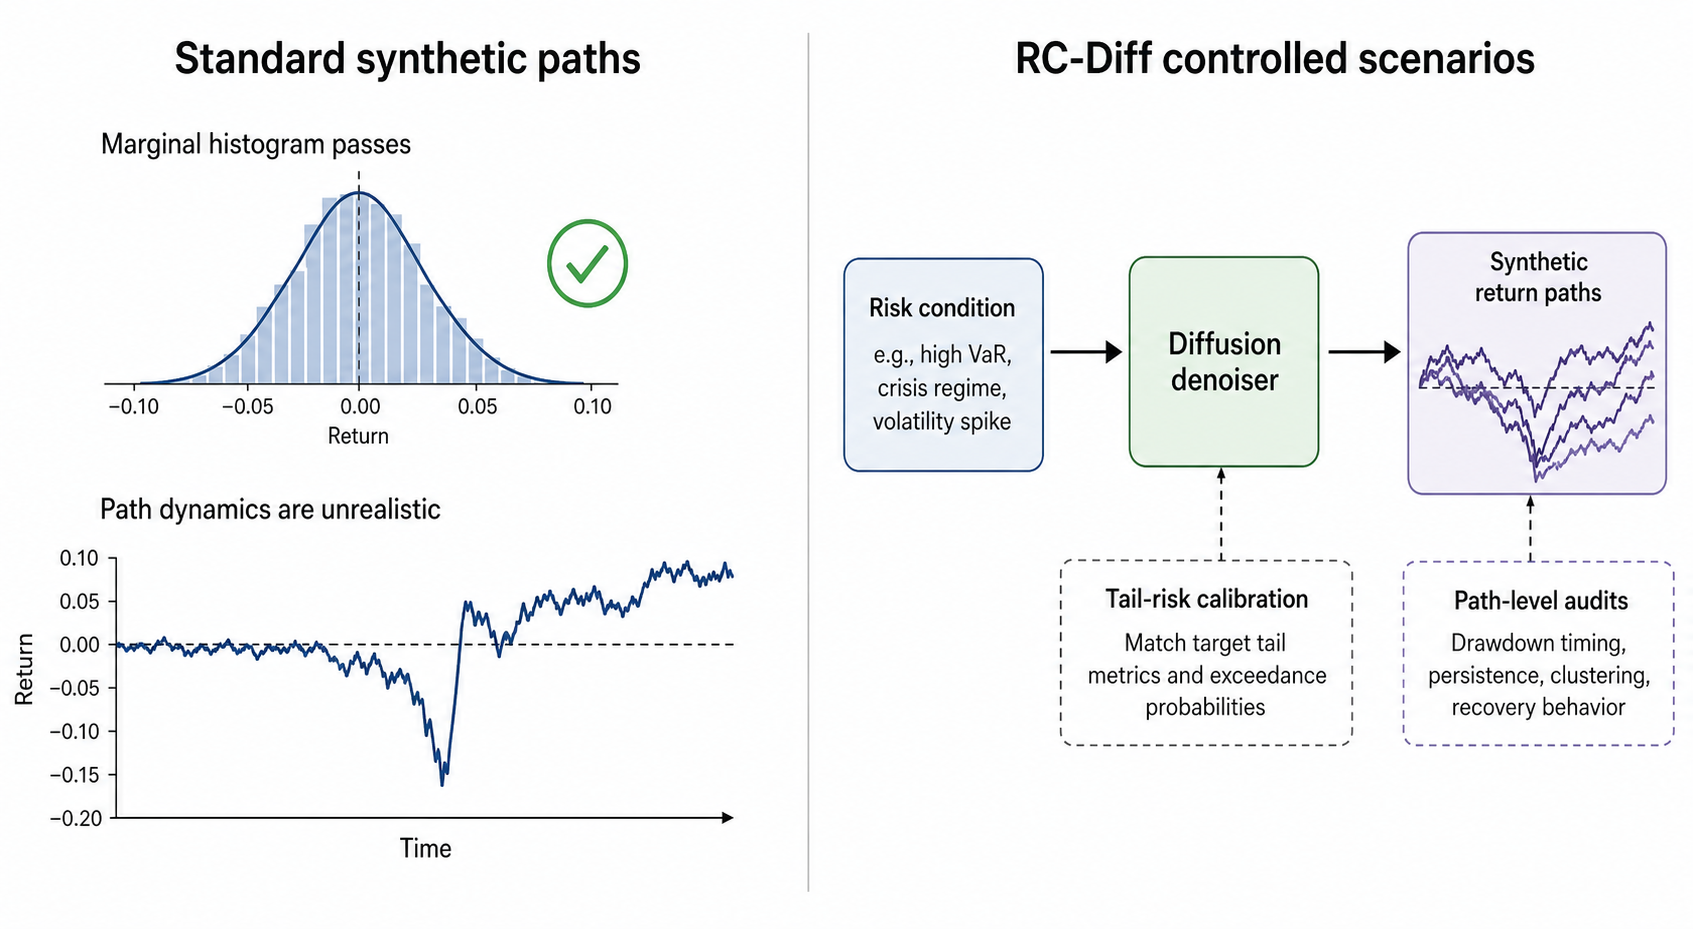
\includegraphics[width=\linewidth]{fig_introduction_teaser.png}
\caption{RC-Diff motivates risk-controlled financial generation: marginally plausible synthetic paths can still fail as stress scenarios, so generated paths are evaluated by both tail-risk calibration and path-level audits.}
\label{fig:introduction_teaser}
\end{figure}

Three findings shape the answer. First, explicit volatility conditioning is effective and diagnostic: shuffled conditioning labels collapse control, while the correctly conditioned model reaches Spearman 0.9788 and low VaR/ES calibration error. Second, signature metrics catch ordering failures that marginal metrics miss; a depth-3 Mahalanobis signature score improves temporal-failure detection AUC by 4.61\% over the strongest marginal-only baseline. Third, simply adding differentiable stylized-fact losses to noisy diffusion reconstructions is harmful in this implementation, increasing tail-index error by 65.4\%. The resulting lesson is practical: risk-aware financial generation should separate controllable risk interfaces, sample-level calibration, and path-level audits, rather than relying on generic auxiliary moment matching.

The main numerical pattern is summarized in the Results section: RC-Diff improves tail-risk calibration, signature audits detect temporal failures better than marginal scores, and the stylized-fact auxiliary loss worsens tail fidelity.

\section{Related Work}
\textbf{Stylized facts and financial risk evaluation.} Empirical finance has long documented that asset returns deviate from Gaussian random walks through heavy tails, volatility clustering, weak raw-return autocorrelation, slow decay in absolute-return autocorrelation, leverage effects, and changing cross-asset dependence \citep{mandelbrot1963variation,ding1993long,engle1993measuring,cont2001stylized}. Conditional-volatility models explain part of this structure through ARCH/GARCH dynamics and asymmetric extensions \citep{engle1982arch,bollerslev1986garch,nelson1991egarch,glosten1993relation}, while stochastic-volatility models offer latent continuous-time alternatives \citep{heston1993closed}. Risk management evaluates generated scenarios through tail-sensitive quantities: VaR, ES, exceedance independence, and joint VaR/ES elicitability/backtesting \citep{artzner1999coherent,kupiec1995techniques,christoffersen1998evaluating,acerbi2002expected,fissler2016higher,nolde2017elicitability}. Our experiments adopt this view by treating volatility control as insufficient unless generated samples also calibrate VaR, ES, and drawdown.

\textbf{Neural time-series generation.} Early neural sequence generators adapted adversarial learning to continuous time series and financial returns. QuantGAN showed that convolutional adversarial models can reproduce several stylized facts in returns \citep{wiese2020quant}. Our comparison follows the broader evaluation principle that synthetic financial paths should be assessed beyond visual realism, but focuses the evaluation on risk controls and path audits.

\textbf{Diffusion models for temporal data.} Diffusion models originate from iterative denoising and score estimation \citep{sohldickstein2015deep,ho2020ddpm,song2021score}. Improved samplers demonstrated that denoising objectives can scale to high-fidelity generation \citep{nichol2021improved}. In financial synthesis, CoFinDiff is closest in spirit because it conditions a diffusion generator on desired financial time-series properties \citep{tanaka2025cofindiff}. Our contribution is complementary: we emphasize empirical calibration of the control channel and failure-detection audits rather than only sample realism.

\textbf{Path signatures and sequence metrics.} Path signatures summarize ordered trajectories through iterated integrals and characterize path laws under suitable conditions \citep{lyons1998differential,chevyrev2016primer,chevyrev2018characteristic}. Signature-based discrepancies are especially relevant for financial generation because marginal distributions can be preserved while order, persistence, and drawdown geometry are corrupted. Sig-Wasserstein GANs use signature-based objectives for time-series generation, and conditional Sig-Wasserstein GANs extend this idea to conditional sequence laws \citep{ni2021sigwgan,liao2023conditional}. We use signature distances not as a training objective in the headline model, but as an audit layer that tests whether evaluation metrics detect temporal corruptions invisible to marginal scores.

\section{Preliminaries}
Let $x_0 \in \mathbb{R}^{T \times d}$ denote a window of log returns for $d$ assets over $T$ trading days. The realized annualized volatility of a univariate path is
\begin{equation}
  \mathrm{RV}(x_0)=\sqrt{252\,T^{-1}\sum_{t=1}^{T} x_{0,t}^2}.
\end{equation}
For multivariate windows we compute the conditioning label from the target asset or aggregate window statistic used in training. The goal is to sample $\hat{x}_0\sim p_\theta(x_0\mid c)$ for a requested risk condition $c$, such that realized sample statistics match the requested regime and held-out real paths.

\textbf{DDPM.} A denoising diffusion probabilistic model defines a fixed forward noising process and a learned reverse denoising process. With variance schedule $\{\beta_k\}_{k=1}^{K}$, $\alpha_k=1-\beta_k$, and $\bar{\alpha}_k=\prod_{s=1}^{k}\alpha_s$, the forward process has the closed form
\begin{equation}
  q(x_k\mid x_0)=\mathcal{N}\!\left(\sqrt{\bar{\alpha}_k}x_0,(1-\bar{\alpha}_k)I\right),
\end{equation}
so a noisy sample can be written as $x_k=\sqrt{\bar{\alpha}_k}x_0+\sqrt{1-\bar{\alpha}_k}\epsilon$ for $\epsilon\sim\mathcal{N}(0,I)$. The network is trained to predict the injected noise and then used to parameterize the reverse transition from $x_k$ to $x_{k-1}$.

\textbf{Conditional diffusion for risk control.} RC-Diff uses the conditional variant of this DDPM: the reverse model is $p_\theta(x_{k-1}\mid x_k,c)$, where $c$ is the requested risk regime. In our implementation, $c$ is standardized realized volatility during training and a user-selected volatility quantile at generation time. The condition is injected into every residual block of the denoiser, so it influences the entire reverse trajectory rather than re-ranking or rescaling samples after generation. This distinction is important for evaluation: the model must transform Gaussian noise into a path whose realized volatility, VaR, ES, and drawdown are consistent with $c$.

We report monotonicity with Spearman correlation between requested and realized volatility across target quantiles, but treat it as insufficient by itself. A model can sort unconditional samples into bins after generation and obtain high rank correlation without learning a useful control channel. We therefore also measure VaR and expected-shortfall calibration error, maximum-drawdown calibration, absolute-return autocorrelation error, tail-index error, and signature-proxy distance.

For path auditing, we compare a generated or corrupted path to a reference set using marginal metrics and signature distances. The signature score is computed on normalized, time-augmented cumulative-return paths at depths 2--4, with either Euclidean or Mahalanobis distance to reference signature moments.

\section{Method}
\begin{figure*}[t]
\centering
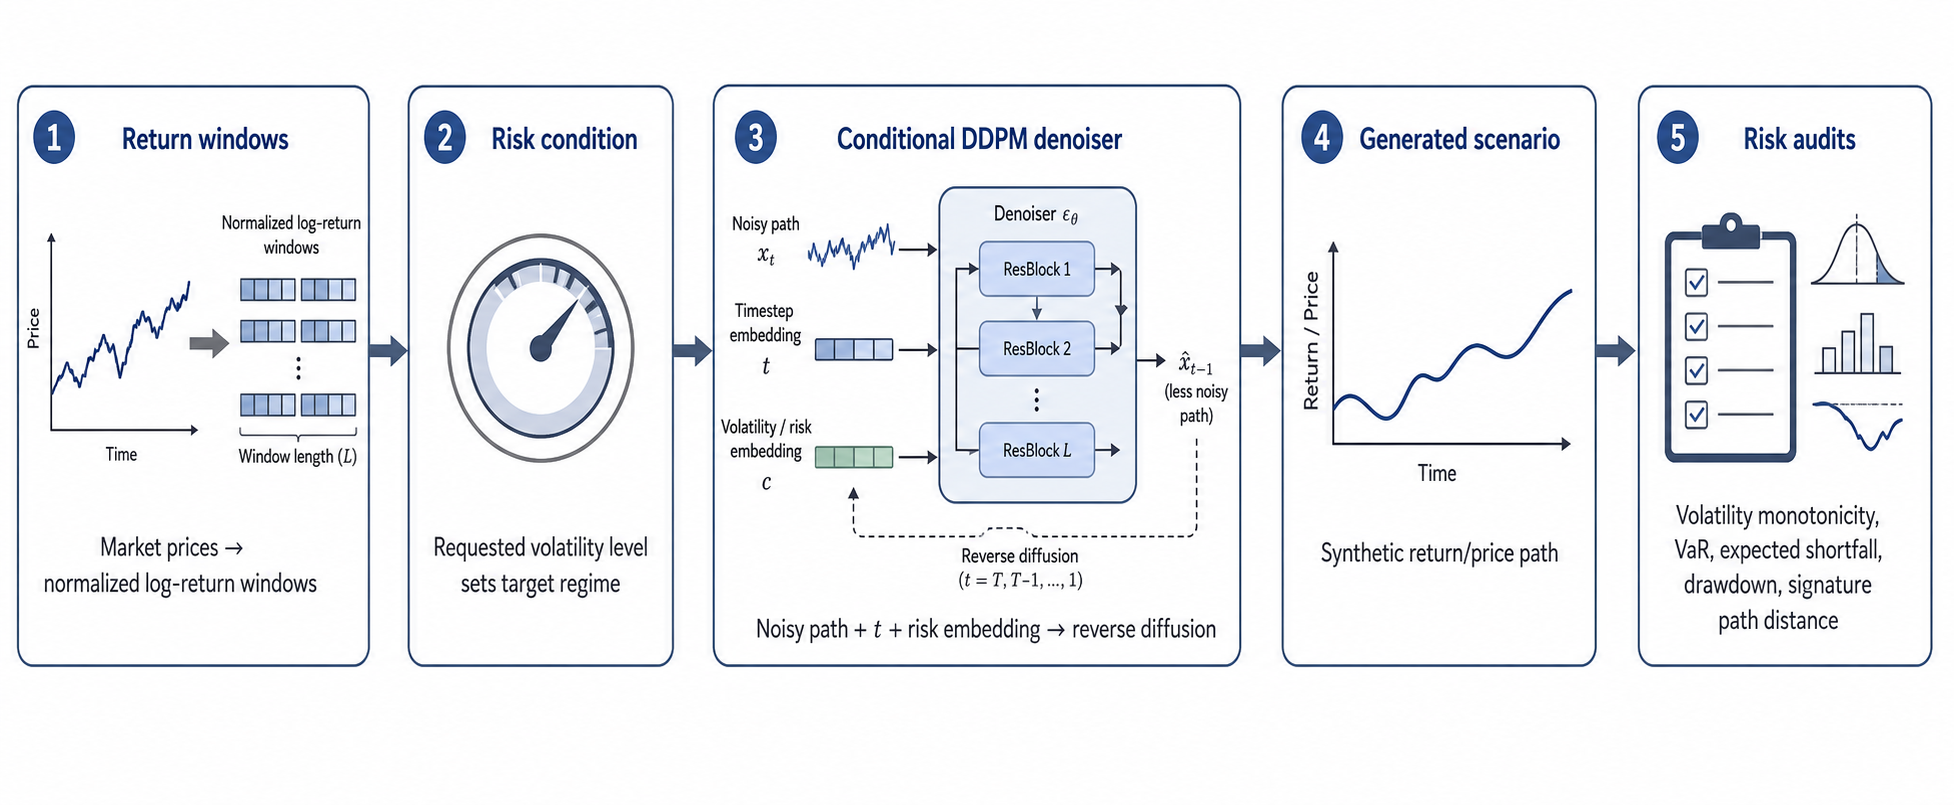
\includegraphics[width=0.92\textwidth]{fig_method_overview.png}
\caption{RC-Diff transforms market prices into controlled synthetic return paths. The volatility condition is injected throughout the DDPM denoiser, and generated paths are evaluated by risk calibration and path-level audits.}
\label{fig:method_overview}
\end{figure*}

\textbf{Problem interface.} Figure~\ref{fig:method_overview} summarizes the input-to-output flow. Each training example is a normalized log-return window $x_0\in\mathbb{R}^{T}$ with $T=64$ in the main control experiment. The conditioning scalar is the window's annualized realized volatility, standardized with the training-set statistics before being passed to the network. The model therefore learns a conditional law $p_\theta(x_0\mid c)$, where $c$ is not an asset identifier or a future label, but the requested risk regime. The end-to-end flow is: raw adjusted prices $\rightarrow$ log returns $\rightarrow$ rolling return windows $\rightarrow$ realized-volatility labels $\rightarrow$ conditional denoising training $\rightarrow$ reverse-diffusion sampling at chosen volatility quantiles $\rightarrow$ risk and path-level audit metrics.

\textbf{Architecture.} The denoiser $\epsilon_\theta(x_t,t,c)$ is a compact one-dimensional U-Net over the time axis. A $3$-wide convolution maps the noisy return path from one channel to 64 hidden channels. Two residual convolutional blocks process the full-resolution sequence, an average-pooling layer halves the temporal resolution, a bottleneck residual block operates at 128 channels, and nearest-neighbor upsampling restores the original length. Skip additions connect the encoder and decoder at matching resolutions. Each residual block uses group normalization, SiLU activations, two width-3 temporal convolutions, and an additive conditioning bias projected from the shared embedding. The output head maps the hidden sequence back to one channel, producing a noise estimate with the same shape as the input return window.

\textbf{Condition injection.} The diffusion timestep is encoded with a sinusoidal embedding and passed through a two-layer MLP. The requested volatility $c$ is passed through a separate two-layer MLP, and the two embeddings are added before being injected into every residual block. This makes the condition global over the whole path: it does not prescribe individual returns, but shifts the denoising dynamics toward paths whose aggregate volatility should match the requested regime. The unconditional ablation removes the volatility MLP and receives only the timestep embedding; the shuffled-label ablation keeps the same architecture but randomly permutes volatility labels during training.

\textbf{Condition construction and use.} The control label is computed only from the window being modeled, then standardized with training-set mean and variance. At sampling time, the user specifies a target volatility quantile, which is converted to the same standardized scale before reverse diffusion begins. We intentionally use a low-dimensional control rather than a learned text prompt or market-regime identifier, because risk managers can audit a scalar volatility request directly against realized volatility, VaR, expected shortfall, and drawdown. The scalar condition also prevents the generator from hiding regime information in opaque side channels: if the requested condition changes, the generated path statistics must move through the denoising vector field.

The condition is held fixed across all reverse steps for a sample, but its effect is not constant. Early denoising steps shape coarse path energy and trend-like cumulative movement; later steps refine local return fluctuations. Injecting the same control embedding into every residual block therefore lets RC-Diff express both low-frequency stress regimes and high-frequency volatility clustering. This differs from post-hoc binning, which samples unconditionally and only sorts outputs after generation. Post-hoc binning can improve rank metrics, but it cannot guarantee that the conditional distribution itself has learned the requested risk law.

\textbf{Forward and reverse diffusion.} We use a DDPM with $K=200$ diffusion steps and a linear variance schedule from $10^{-4}$ to $0.02$. Given a clean return window $x_0$, a timestep $k$, and Gaussian noise $\epsilon\sim\mathcal{N}(0,I)$, the forward process is
\begin{equation}
  x_k=\sqrt{\bar{\alpha}_k}x_0+\sqrt{1-\bar{\alpha}_k}\epsilon,
\end{equation}
where $\bar{\alpha}_k=\prod_{s=1}^k(1-\beta_s)$. The network predicts $\epsilon$ from $(x_k,k,c)$. At generation time, sampling starts from $x_K\sim\mathcal{N}(0,I)$ and iterates the standard DDPM reverse mean
\begin{equation}
  \mu_\theta(x_k,k,c)=\frac{1}{\sqrt{\alpha_k}}\left(x_k-\frac{\beta_k}{\sqrt{1-\bar{\alpha}_k}}\epsilon_\theta(x_k,k,c)\right),
\end{equation}
adding Gaussian posterior noise for $k>1$. The output is a complete synthetic return path $\hat{x}_0$, which can be cumulatively summed into a price-relative scenario for drawdown and stress-test metrics.

\textbf{Training objective.} The base objective is the denoising score-matching loss
\begin{equation}
  \mathcal{L}_{\mathrm{DDPM}}=\mathbb{E}_{x_0,c,k,\epsilon}\left[\|\epsilon-\epsilon_\theta(x_k,k,c)\|_2^2\right].
\end{equation}
Models are trained with AdamW at learning rate $2\times10^{-4}$, batch size 256, gradient clipping at 1.0, and 6,000 optimization steps for diffusion variants. This objective is intentionally simple: all risk awareness enters through the conditioning channel and through evaluation, not through hand-tuned postprocessing of samples.

\textbf{Sampling protocol.} For each requested quantile, RC-Diff draws independent Gaussian initial states and applies the same reverse chain with the chosen condition. We generate multiple paths per condition rather than optimizing a single representative path, because financial stress testing requires a distribution of plausible futures around a requested risk level. After sampling, generated returns are left in return space for statistical evaluation and cumulatively summed only for drawdown and path-visualization metrics. No sample is rejected, clipped, or rescaled after generation; this is essential for interpreting calibration errors as properties of the learned conditional model rather than artifacts of postprocessing.

\textbf{Training objective design.} The denoising loss is evaluated at uniformly sampled diffusion steps, so the network must learn both high-noise global reconstruction and low-noise local refinement. This matters for financial data because tail events and volatility clustering appear at different scales. A high-noise step mainly determines the energy and direction of the whole window, while a low-noise step determines whether large returns cluster realistically. RC-Diff keeps the primary objective at the noise-prediction level to preserve the likelihood-based DDPM training signal, then reserves most stylized-fact checks for evaluation where they can be measured on final samples.

\textbf{Stylized-fact auxiliary objective.} For the stylized-fact-loss ablation, we additionally reconstruct $\hat{x}_0=(x_k-\sqrt{1-\bar{\alpha}_k}\epsilon_\theta(x_k,k,c))/\sqrt{\bar{\alpha}_k}$ and penalize mismatches between $\hat{x}_0$ and $x_0$ in volatility, mean absolute return, absolute-return autocorrelation at lags 1 and 5, and a Hill-style tail proxy. In compact form,
\begin{equation}
  \mathcal{L}=\mathcal{L}_{\mathrm{DDPM}}+\lambda_{\mathrm{SF}}\sum_j d_j(f_j(\hat{x}_0),f_j(x_0)),
\end{equation}
where $f_j$ are stylized-fact statistics and $d_j$ are squared errors. The negative ablation result shows why we keep this loss out of the headline model: statistics computed from noisy reconstructions can supply biased gradients that improve one proxy while damaging tails, correlations, or signature distance.

\textbf{Risk calibration.} The primary control check compares requested volatility bins with realized volatility in generated samples. Calibration is assessed with VaR, expected shortfall, and maximum-drawdown errors against held-out or benchmark targets. A model is considered useful only if the control is both monotone and calibrated: increasing $c$ should increase realized volatility, but the generated samples should also land near the requested tail-risk regime rather than merely sort samples by variance.

\begin{theorem}[Monotone control under calibrated conditional diffusion]
\label{thm:monotone-control}
Let $c_1<c_2$ be two volatility conditions. Suppose the learned reverse DDPM transitions equal the true conditional reverse transitions for $p(x_0\mid c)$, and suppose the training conditional laws are ordered so that $\mathrm{RV}(X_0\mid c_2)$ first-order stochastically dominates $\mathrm{RV}(X_0\mid c_1)$. Then samples $\hat{X}_0(c)$ produced by the conditional reverse chain satisfy
\begin{equation}
  \mathbb{E}[\mathrm{RV}(\hat{X}_0(c_2))]\geq \mathbb{E}[\mathrm{RV}(\hat{X}_0(c_1))].
\end{equation}
Moreover, for any threshold $u$, $\Pr[\mathrm{RV}(\hat{X}_0(c_2))\geq u]\geq \Pr[\mathrm{RV}(\hat{X}_0(c_1))\geq u]$.
\end{theorem}

The theorem does not claim that any finite neural implementation is automatically monotone. Rather, it formalizes the ideal control target by combining the DDPM consistency premise of learned reverse transitions \citep{ho2020ddpm,song2021score} with the financial premise that realized volatility indexes ordered risk regimes \citep{engle1982arch,bollerslev1986garch,mcneil2015quantitative}. Under those two assumptions, monotonicity is a property of the conditional law, not a post-processing trick. This is why RC-Diff evaluates both rank ordering and risk-unit calibration: the Spearman score tests the stochastic-order implication, while VaR/ES and drawdown errors test whether the generated conditional law is close enough for risk use \citep{artzner1999coherent,acerbi2002expected,fissler2016higher}. The shuffled-label ablation is the direct falsification test: it preserves the U-Net and DDPM objective but destroys the empirical coupling between $x_0$ and $c$, so the theorem's ordered-law premise should fail.

\begin{proposition}[Global conditioning changes path-level statistics]
\label{prop:conditioning-flow}
Consider a reverse DDPM whose mean has the form in Eq.~(4), and suppose the denoiser is differentiable in a scalar condition $c$. Let $S:\mathbb{R}^{T}\rightarrow\mathbb{R}$ be any differentiable path statistic, such as realized volatility after smoothing by $\delta>0$, $S_\delta(x)=\sqrt{252T^{-1}\sum_t x_t^2+\delta}$. If there is at least one reverse step $k$ for which
\begin{equation}
\begin{split}
  \mathbb{E}\Big[\nabla_x S_\delta(X_{k-1})^\top
  \frac{\partial \mu_\theta(X_k,k,c)}{\partial c}\Big]\neq0 .
\end{split}
\end{equation}
then changing $c$ changes the expected generated statistic to first order:
\begin{equation}
  \frac{d}{dc}\mathbb{E}[S_\delta(\hat{X}_0(c))]\neq0
\end{equation}
for the composed reverse chain, except in degenerate cancellations across later steps.
\end{proposition}

This proposition connects the architecture to the control interface. Conditional diffusion models alter the reverse denoising distribution rather than fitting a separate generator per regime \citep{tanaka2025cofindiff}; in RC-Diff, the volatility embedding enters every residual block so $\partial\mu_\theta/\partial c$ can be nonzero at multiple resolutions and diffusion times. The result says that if these local condition derivatives align with the gradient of a path statistic such as smoothed realized volatility, then the expected statistic must move to first order through the composed reverse chain. This gives a mechanistic explanation for the empirical gap between correctly labeled conditioning and shuffled labels: correct labels create a stable direction in the denoising vector field, while shuffled labels train condition derivatives that average toward zero or conflict across regimes.

\begin{proposition}[Noisy auxiliary statistics can bias denoising]
\label{prop:noisy-stat-bias}
Let $f$ be a nonlinear stylized-fact statistic and let $\hat{x}_0(k)=a_k x_0+b_k\eta$ be a reconstruction observed inside a diffusion step, where $0<a_k<1$, $b_k>0$, and $\eta$ is zero-mean noise independent of $x_0$. In general,
\begin{equation}
  \nabla_\theta\mathbb{E}\left[(f(\hat{x}_0(k))-f(x_0))^2\right]
\end{equation}
is not an unbiased gradient for reducing the sample-level discrepancy $\mathbb{E}[(f(\tilde{x}_0)-f(x_0))^2]$ of final generated samples $\tilde{x}_0\sim p_\theta(\cdot\mid c)$. The mismatch contains attenuation terms from $a_k$, curvature terms from $f$, and noise terms scaling with $b_k^2$.
\end{proposition}

Proposition~\ref{prop:noisy-stat-bias} gives a theoretical reason for the negative stylized-fact-loss ablation. The failed auxiliary objective computes tail, autocorrelation, and volatility penalties on noisy single-step reconstructions, not on final low-noise samples. For heavy-tail and autocorrelation statistics, this can push the denoiser toward proxy values that are easier under the corrupted reconstruction distribution but worse under the final reverse chain. RC-Diff therefore treats stylized facts mainly as calibration and audit targets, while the trainable control mechanism remains the conditional DDPM objective.

\textbf{Signature audit.} To test whether evaluation sees path ordering, we create controlled corruptions of held-out real windows: full shuffling, block shuffling, sign shuffling, and time reversal. These preserve much of the marginal return distribution while damaging temporal structure. Metrics are scored by paired ROC-AUC for distinguishing real from corrupted paths. The signature features are computed on time-augmented cumulative-return paths and compared with reference moments using Euclidean or Mahalanobis distances, giving an audit layer independent of the diffusion training loss.

\section{Experiments}
\subsection{Setup}
The main control experiment uses daily OHLCV data downloaded from Yahoo Finance for 41 large-cap S\&P 500 constituents and SPY over 2010--2024. Returns are converted to rolling 64-day log-return windows, giving 37,709 S\&P 500 windows and 928 SPY windows. The model generates 500 samples for each requested volatility quantile: 10, 25, 50, 75, and 90 percent.

Baselines follow the main comparison frame: TimeGAN-lite, C-RNN-GAN-lite, a conditional Sig-Wasserstein GAN proxy, an unconditional diffusion with post-hoc volatility binning, and a diffusion ablation without stylized-fact loss. The Sig-Wasserstein GAN proxy uses a conditional GRU generator and discriminator with truncated cumulative-signature moment matching. Metrics include Spearman control correlation, monotonicity violations, VaR/ES/max-drawdown calibration, absolute-return autocorrelation, signature-proxy distance, and tail-index error.

A separate path-audit experiment uses 95 liquid S\&P 500 constituents over 2010--2024. It builds 128-day rolling adjusted-close return windows with stride 64, using 3,230 pre-2019 reference windows and 2,090 held-out 2019--2024 windows. We compare six marginal metrics, two autocorrelation-profile metrics, and six signature metrics.

\subsection{Main Results}
Table~\ref{tab:main} reports the headline risk-control comparison. The central experimental question is whether the conditioning variable used by RC-Diff changes the generated path distribution in risk units, rather than merely sorting samples after generation. Rank monotonicity alone is deceptive: TimeGAN, C-RNN-GAN, and unconditional diffusion achieve high Spearman values after post-hoc binning. Their calibration errors show the difference. RC-Diff has the best VaR and ES calibration and maintains zero monotonicity violations. The Sig-Wasserstein GAN proxy, the closest conditional baseline, fails the control task with Spearman 0.0171 and a 0.5 violation rate.

\begin{figure}[t]
\centering

\includegraphics[width=\linewidth]{hypotheses/H2/fig1_spearman.png}
\caption{Volatility-control check. Correct RC-Diff conditioning gives monotone realized volatility, while shuffled labels and the conditional adversarial baseline fail the ordered-control test.}
\label{fig:volatility_control}
\end{figure}

\begin{table*}[t]
\centering
\caption{Main volatility-control results on Yahoo Finance S\&P 500 return windows. Lower is better except Spearman.}
\label{tab:main}
\resizebox{\textwidth}{!}{%
\begin{tabular}{lrrrrrr}
\toprule
Method & Spearman & Viol. & VaR err. & ES err. & MDD err. & Tail err. \\
\midrule
TimeGAN-lite & 0.9798 & 0.0000 & 10.5525 & 7.7718 & 75.8714 & 2.2990 \\
C-RNN-GAN-lite & 0.9798 & 0.0000 & 0.5823 & 0.6046 & 0.6670 & 0.7883 \\
Sig-W-GAN-lite & 0.0171 & 0.5000 & 0.9043 & 0.9162 & 0.2857 & 1.5580 \\
Uncond. diffusion + bins & 0.9798 & 0.0000 & 0.3747 & 0.4145 & 0.6304 & 0.1643 \\
RC-Diff, no SF loss & 0.9772 & 0.0000 & 0.1748 & 0.0685 & \textbf{0.1821} & \textbf{0.0716} \\
RC-Diff & 0.9788 & 0.0000 & \textbf{0.1454} & \textbf{0.0499} & 0.2069 & 0.0969 \\
\bottomrule
\end{tabular}%
}
\end{table*}

\begin{figure}[t]
\centering

\includegraphics[width=\linewidth]{hypotheses/H2/fig2_calib.png}
\caption{Tail-risk calibration. RC-Diff is evaluated in VaR and expected-shortfall units because the method is designed for calibrated financial stress generation.}
\label{fig:risk_calibration}
\end{figure}

The shuffled-label ablation confirms that the conditioning signal is real. With randomly permuted volatility labels, Spearman drops to $-0.0056$ and monotonicity violations rise to 0.4583. VaR and ES calibration errors also worsen to 0.5110 and 0.6443. The learned control channel is therefore not just an unconditional volatility mixture, as visualized by Figure~\ref{fig:volatility_control}.

\subsection{Ablations and Analyses}
\textbf{Stylized-fact loss.} Table~\ref{tab:sf} and Figure~\ref{fig:stylized_ablation} test whether financial stylized facts should be imposed as an auxiliary training objective or reserved for evaluation. On 16 liquid S\&P 500 names from 2010--2024, with a train/test split at 2022, the no-loss diffusion reaches tail-index error 1.448. Adding Hill, absolute-autocorrelation, and correlation losses on $\hat{x}_0$ increases tail-index error to 2.396, with one-sided Wilcoxon $p=1.0$ for the intended improvement. Correlation distance and signature distance also deteriorate. This matches Proposition~\ref{prop:noisy-stat-bias}: at moderate diffusion noise, $\hat{x}_0$ is a biased proxy for the final sample, so moment-matching gradients can pull against denoising.

\begin{table}[t]
\centering
\caption{Stylized-fact loss ablation. Lower is better.}
\label{tab:sf}
\begin{tabular}{lrrrr}
\toprule
Method & Tail & $|r|$ ACF & Corr. & SigW \\
\midrule
SeqGAN & 92.6066 & 0.4509 & 10.3545 & 0.0116 \\
RC-Diff, no SF & \textbf{1.4484} & 0.0320 & \textbf{1.7096} & \textbf{0.0011} \\
RC-Diff + SF & 2.3961 & \textbf{0.0313} & 5.5547 & 0.0188 \\
\bottomrule
\end{tabular}
\end{table}

\begin{figure*}[t]
\centering
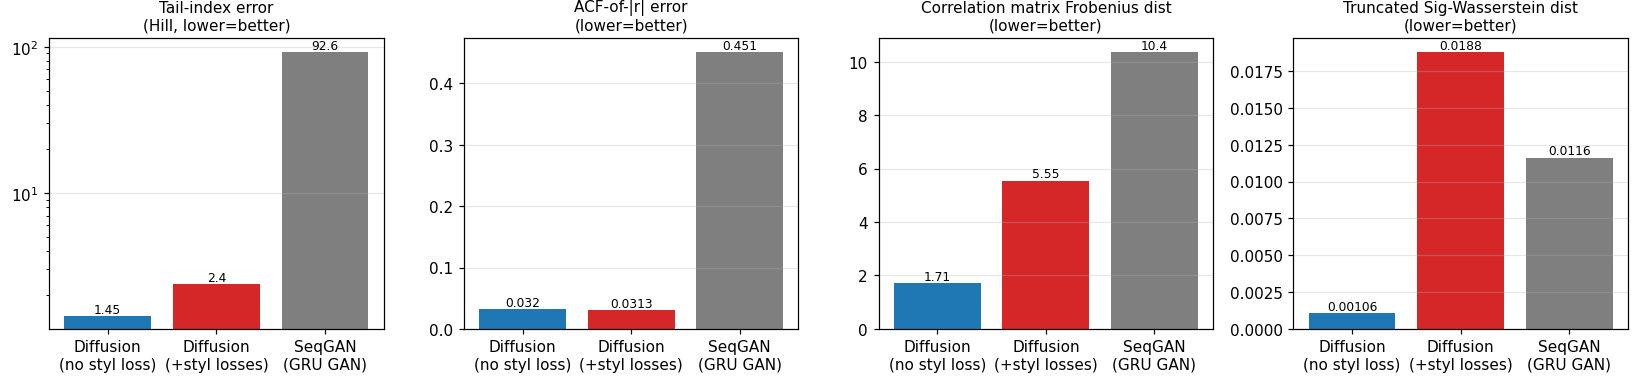
\includegraphics[width=0.95\textwidth]{fig_stylized_ablation.png}
\caption{Stylized-loss ablation. Penalizing noisy reconstructions worsens final-sample tail fidelity and signature distance, supporting the decision to use stylized facts as audits.}
\label{fig:stylized_ablation}
\end{figure*}

\textbf{Path-level audit.} Table~\ref{tab:audit} evaluates whether RC-Diff samples preserve temporal ordering beyond marginal return realism. These rows are audit metrics rather than generator names: SigW Maha depth 3 denotes a signature-Wasserstein score using Mahalanobis normalization and depth-3 path signatures. The audit deliberately corrupts ordering while preserving many pointwise statistics, so success means the score is sensitive to the path structure that the generator is supposed to model.

\begin{table}[t]
\centering
\caption{Temporal-failure detection AUC on RC-Diff samples. Higher is better.}
\label{tab:audit}
\resizebox{\linewidth}{!}{%
\begin{tabular}{lr}
\toprule
RC-Diff audit metric & Mean paired AUC \\
\midrule
KS & 0.5182 \\
Wasserstein-1 & 0.5163 \\
Tail Hill error & 0.5000 \\
VaR5 error & 0.4947 \\
ES5 error & 0.5023 \\
Gaussian MMD & 0.5404 \\
Abs-ACF Mahalanobis & 0.4965 \\
Sign-ACF Mahalanobis & 0.5007 \\
SigW L2 depth 3 & 0.5590 \\
SigW L2 depth 4 & 0.5599 \\
SigW Maha depth 3 & \textbf{0.5657} \\
SigW Maha depth 4 & 0.5607 \\
\bottomrule
\end{tabular}%
}
\end{table}

Gaussian MMD is the strongest marginal-only baseline with mean paired AUC 0.5404, mostly from sign shuffle. The best RC-Diff audit metric, SigW Maha depth 3, reaches AUC 0.5657, a 4.61\% relative gain with 95\% bootstrap confidence interval [1.53, 7.68]. On the strictly marginal-blind subset of full shuffle, block shuffle, and time reversal, marginal metrics collapse to chance around 0.500 while signature metrics reach roughly 0.543--0.556. This audit closes the loop with the method: RC-Diff generates full paths, so the evaluation must test ordering, regime persistence, and drawdown dynamics rather than only one-step return histograms.

\textbf{Sensitivity.} Table~\ref{tab:audit} also shows that signature depth matters, and the improvement is not an artifact of one corruption type. Depth-2 variants are weaker and do not consistently clear the improvement threshold, while depth 3 and depth 4 are reliable. Depth-3 Mahalanobis is strongest, suggesting that moderate-depth signatures capture useful ordering information without excessive estimation noise. Runtime is practical: all six signature scores cost about 12 ms per window, compared with about 110 ms for the marginal metric suite dominated by empirical MMD.

\textbf{Case study.} High-volatility requested samples are useful when they are calibrated rather than merely volatile. In the control experiment, the conditioned diffusion reduces VaR/ES errors relative to unconditional diffusion by 0.2293 and 0.3646 absolute points. This is the practical difference between a stress generator that can rank requested regimes and one that lands closer to the actual target risk level.

The case study also illustrates how RC-Diff should be used as a deployment checklist rather than as a sample visualizer. A risk desk would first request a volatility regime, then verify monotonic response, tail-risk calibration, and path-level plausibility before using the generated paths in a stress test. The three experiment blocks map directly to those checks: Figure~\ref{fig:volatility_control} tests whether the control channel moves realized volatility in the requested order, Table~\ref{tab:main} tests whether VaR and expected shortfall land in calibrated risk units, and Table~\ref{tab:audit} tests whether temporal-order failures are visible to signature audits. The failed stylized-loss ablation is part of the same case study because it prevents a tempting but unsafe shortcut: directly penalizing noisy reconstructions can improve a proxy statistic while making final samples less faithful.

This workflow keeps the method falsifiable when richer controls are added. A drawdown, liquidity, or cross-market stress knob should be accepted only if it passes the same three linked quantities: the requested regime, the realized risk statistic, and an order-sensitive path audit. In this sense the current equity-volatility experiment is deliberately narrow. It validates the control channel and audit protocol before adding more expressive conditioning variables whose failures would be harder to diagnose.

\section{Conclusion}
RC-Diff frames financial time-series diffusion as controlled risk generation rather than generic sequence synthesis. Explicit volatility conditioning gives monotone and better-calibrated equity-return paths, while shuffled labels show that the control channel is actually used. Signature distances add a path-level audit for temporal failures that marginal metrics miss, and the stylized-loss ablation shows why financial facts are safer as final-sample audits than as noisy-time penalties.

Future work should move stylized-fact objectives to low-noise or sample-level training, extend conditioning from volatility to joint drawdown and tail-severity controls, and test regime-shift generalization on crisis-period holdouts.

\begin{thebibliography}{99}

\bibitem[Acerbi and Tasche(2002)]{acerbi2002expected} Acerbi, C. and Tasche, D. (2002). On the coherence of expected shortfall. \emph{Journal of Banking \& Finance}.
\bibitem[Artzner et~al.(1999)]{artzner1999coherent} Artzner, P., Delbaen, F., Eber, J.-M., and Heath, D. (1999). Coherent measures of risk. \emph{Mathematical Finance}.
\bibitem[Bollerslev(1986)]{bollerslev1986garch} Bollerslev, T. (1986). Generalized autoregressive conditional heteroskedasticity. \emph{Journal of Econometrics}.
\bibitem[Chevyrev and Kormilitzin(2016)]{chevyrev2016primer} Chevyrev, I. and Kormilitzin, A. (2016). A primer on the signature method in machine learning. arXiv preprint.
\bibitem[Chevyrev and Lyons(2016)]{chevyrev2018characteristic} Chevyrev, I. and Lyons, T. (2016). Characteristic functions of measures on geometric rough paths. \emph{Annals of Probability}.
\bibitem[Christoffersen(1998)]{christoffersen1998evaluating} Christoffersen, P. F. (1998). Evaluating interval forecasts. \emph{International Economic Review}.
\bibitem[Cont(2001)]{cont2001stylized} Cont, R. (2001). Empirical properties of asset returns: stylized facts and statistical issues. \emph{Quantitative Finance}.
\bibitem[Ding et~al.(1993)]{ding1993long} Ding, Z., Granger, C. W. J., and Engle, R. F. (1993). A long memory property of stock market returns and a new model. \emph{Journal of Empirical Finance}.
\bibitem[Embrechts et~al.(1997)]{embrechts1997modelling} Embrechts, P., Klueppelberg, C., and Mikosch, T. (1997). \emph{Modelling Extremal Events for Insurance and Finance}. Springer.
\bibitem[Engle(1982)]{engle1982arch} Engle, R. F. (1982). Autoregressive conditional heteroscedasticity with estimates of the variance of United Kingdom inflation. \emph{Econometrica}.
\bibitem[Engle and Ng(1993)]{engle1993measuring} Engle, R. F. and Ng, V. K. (1993). Measuring and testing the impact of news on volatility. \emph{Journal of Finance}.
\bibitem[Fissler and Ziegel(2016)]{fissler2016higher} Fissler, T. and Ziegel, J. F. (2016). Higher order elicitability and Osband's principle. \emph{Annals of Statistics}.
\bibitem[Glosten et~al.(1993)]{glosten1993relation} Glosten, L. R., Jagannathan, R., and Runkle, D. E. (1993). On the relation between expected value and volatility of nominal excess stock returns. \emph{Journal of Finance}.
\bibitem[Heston(1993)]{heston1993closed} Heston, S. L. (1993). A closed-form solution for options with stochastic volatility. \emph{Review of Financial Studies}.
\bibitem[Ho et~al.(2020)]{ho2020ddpm} Ho, J., Jain, A., and Abbeel, P. (2020). Denoising diffusion probabilistic models. \emph{NeurIPS}.
\bibitem[Kupiec(1995)]{kupiec1995techniques} Kupiec, P. H. (1995). Techniques for verifying the accuracy of risk measurement models. \emph{Journal of Derivatives}.
\bibitem[Liao et~al.(2023)]{liao2023conditional} Liao, S., Ni, H., Szpruch, L., Wiese, M., Sabate-Vidales, M., and Xiao, B. (2023). Sig-Wasserstein GANs for conditional time series generation. \emph{Mathematical Finance}.
\bibitem[Lyons(1998)]{lyons1998differential} Lyons, T. J. (1998). Differential equations driven by rough signals. \emph{Revista Matematica Iberoamericana}.
\bibitem[Mandelbrot(1963)]{mandelbrot1963variation} Mandelbrot, B. (1963). The variation of certain speculative prices. \emph{Journal of Business}.
\bibitem[McNeil et~al.(2015)]{mcneil2015quantitative} McNeil, A. J., Frey, R., and Embrechts, P. (2015). \emph{Quantitative Risk Management}. Princeton University Press.
\bibitem[Nelson(1991)]{nelson1991egarch} Nelson, D. B. (1991). Conditional heteroskedasticity in asset returns: a new approach. \emph{Econometrica}.
\bibitem[Ni et~al.(2021)]{ni2021sigwgan} Ni, H., Szpruch, L., Wiese, M., Liao, S., and Xiao, B. (2021). Sig-Wasserstein GANs for time series generation. \emph{ACM ICAIF}.
\bibitem[Nichol and Dhariwal(2021)]{nichol2021improved} Nichol, A. Q. and Dhariwal, P. (2021). Improved denoising diffusion probabilistic models. \emph{ICML}.
\bibitem[Nolde and Ziegel(2017)]{nolde2017elicitability} Nolde, N. and Ziegel, J. F. (2017). Elicitability and backtesting. \emph{Annals of Applied Statistics}.
\bibitem[Sohl-Dickstein et~al.(2015)]{sohldickstein2015deep} Sohl-Dickstein, J., Weiss, E. A., Maheswaranathan, N., and Ganguli, S. (2015). Deep unsupervised learning using nonequilibrium thermodynamics. \emph{ICML}.
\bibitem[Song et~al.(2021)]{song2021score} Song, Y. et~al. (2021). Score-based generative modeling through stochastic differential equations. \emph{ICLR}.
\bibitem[Tanaka et~al.(2025)]{tanaka2025cofindiff} Tanaka, Y., Hashimoto, Y., et~al. (2025). CoFinDiff: controllable financial diffusion model for time series generation. arXiv preprint.
\bibitem[Wiese et~al.(2020)]{wiese2020quant} Wiese, M., Knobloch, R., Korn, R., and Kretschmer, P. (2020). Quant GANs: deep generation of financial time series. \emph{Quantitative Finance}.

\end{thebibliography}

\appendix
\section{Proof of Theorem~\ref{thm:monotone-control}}
Let $P_c$ be the true law of $X_0\mid c$ and $\hat{P}_c$ the law produced by the learned conditional reverse chain. In the exact DDPM/score-model limit, learned reverse transitions recover the conditional data reverse process, so $\hat{P}_c=P_c$ for each condition \citep{ho2020ddpm,song2021score}. Thus $Z_c=\mathrm{RV}(X_0)$ and $\hat Z_c=\mathrm{RV}(\hat X_0(c))$ have the same distribution. The financial assumption is first-order stochastic dominance of volatility regimes: for $c_2>c_1$, $\Pr[Z_{c_2}\ge u]\ge\Pr[Z_{c_1}\ge u]$ for all $u$, matching the ARCH/GARCH view that regimes order squared-return scale \citep{engle1982arch,bollerslev1986garch}. Equality of true and generated conditional laws transfers this inequality to $\hat Z_c$. Since RV is nonnegative, the layer-cake identity gives $\mathbb{E}\hat Z_c=\int_0^\infty\Pr[\hat Z_c\ge u]du$, and integration proves $\mathbb{E}\hat Z_{c_2}\ge\mathbb{E}\hat Z_{c_1}$. Methodologically, the proof explains why RC-Diff reports both Spearman monotonicity and VaR/ES calibration: the former tests the ordering implication, while the latter checks risk-unit closeness of the conditional law \citep{artzner1999coherent,acerbi2002expected,fissler2016higher}. Shuffled labels remove the ordered-law premise while preserving the architecture.

\section{Proof of Proposition~\ref{prop:conditioning-flow}}
Write one reverse step as $X_{k-1}=\mu_\theta(X_k,k,c)+\sigma_kZ_k$. The condition affects generation only through the reverse mean, so define $J_k=\partial\mu_\theta/\partial x$ and $g_k=\partial\mu_\theta/\partial c$. If $c$ were used only for post-hoc binning, every $g_k$ during generation would be zero; RC-Diff instead injects $c$ into every residual block so $g_k$ may be nonzero across noise levels and resolutions. For smoothed $S_\delta$, pathwise differentiation gives $\partial X_{k-1}/\partial c=J_k\partial X_k/\partial c+g_k$. Because $X_K$ is independent Gaussian noise,
\begin{equation}
  \frac{\partial X_0}{\partial c}=\sum_{k=1}^{K}\left(\prod_{s=1}^{k-1}J_s\right)g_k,
\end{equation}
and therefore
\begin{equation}
  \frac{d}{dc}\mathbb{E}S_\delta(\hat{X}_0(c))=\sum_{k=1}^{K}\mathbb{E}\left[\nabla S_\delta(X_0)^\top\left(\prod_{s=1}^{k-1}J_s\right)g_k\right].
\end{equation}
A nonzero transported term changes the expected path statistic unless later reverse steps cancel it exactly. This proves the proposition and connects directly to the architecture: conditioning throughout the U-Net gives many opportunities for the denoising vector field to align with volatility gradients, whereas shuffled labels make those derivatives inconsistent and empirically collapse control.

\section{Proof of Proposition~\ref{prop:noisy-stat-bias}}
The auxiliary loss evaluates $f$ on $\hat X_0(k)=a_kX_0+b_k\eta$, but calibration evaluates final samples $\tilde X_0\sim p_\theta(\cdot\mid c)$. DDPM noise schedules attenuate signal and add Gaussian corruption at intermediate steps \citep{ho2020ddpm,nichol2021improved}. For nonlinear $f$,
\begin{equation}
\resizebox{\linewidth}{!}{$\displaystyle
  f(a_kX_0+b_k\eta)=f(a_kX_0)+b_k\nabla f(a_kX_0)^\top\eta+\frac{b_k^2}{2}\eta^\top\nabla^2f(a_kX_0)\eta+R_3.
$}
\end{equation}
The zero-mean noise removes the linear term in expectation, but curvature and higher-order terms remain. Even for quadratic volatility, $\mathbb{E}_\eta T^{-1}\|a_kX_0+b_k\eta\|^2=a_k^2T^{-1}\|X_0\|^2+b_k^2T^{-1}\mathbb{E}\|\eta\|^2$, so the statistic is simultaneously shrunk and noise-inflated. Tail, quantile, VaR/ES, autocorrelation, and signature statistics are more biased because they are nonlinear, rare-event, ratio, or path-order functionals \citep{embrechts1997modelling,mcneil2015quantitative,kupiec1995techniques,chevyrev2016primer}. Thus the auxiliary gradient targets the corrupted reconstruction law, not the final clean conditional law. It is unbiased only in special cases such as $b_k=0$, $a_k=1$, affine $f$, or identical one-step and final-sample distributions. This explains the negative stylized-fact-loss ablation: stylized-fact penalties at moderate noise can improve local proxies while worsening final tail and signature metrics, so RC-Diff uses stylized facts for calibration/audit and keeps sampling trained by conditional denoising.

\end{document}

